\documentclass[twoside,        %% zweiseitiges Layout
			   12pt,			%% Zeilenabstand
               BCOR10mm,       %% Bindekorrektur 10 mm
%               liststotoc,nomtotoc,bibtotoc, %% Aufnahme der div. Verzeichnisse
                                              %% ins Inhaltsverzeichnis
              % english,ngerman, %% Alternativspr. Englisch, Dokumentspr. Deutsch
               ngerman,english  %% Alternativspr. Deutsch, Dokumentspr. Englisch
%               final,          %% Endversion; draft fuer schnelles Kompilieren
%				smallheadings,
               ]{scrartcl}

\usepackage{tikz}
\usetikzlibrary{shapes,arrows,fit,calc,positioning}
\usepackage{setspace}  %% Zur Setzung des Zeilenabstandes
\usepackage[english,ngerman]{babel}     %% Sprachen-Unterstuetzung
\usepackage{calc}      %% ermoeglicht Rechnen mit Laengen und Zaehlern
\usepackage[T1]{fontenc}       %% Unterstutzung von Umlauten etc.
%\usepackage[latin1]{inputenc}  %% 
%% in aktuellem Linux & MacOS X wird standardmaessig UTF8 kodiert!
\usepackage[utf8]{inputenc}    %% Wenn latin1 nicht geht ...
\usepackage{subfigure}

\usepackage{amsmath,amssymb} %% zusaetzliche Mathe-Symbole

\usepackage{lmodern} %% type1-taugliche CM-Schrift als Variante zur
                     %% "normalen" EC-Schrift
%% Paket fuer bibtex-Datenbanken
\usepackage[comma,numbers,sort&compress]{natbib}
\bibliographystyle{plainnat}

\newcommand{\tabheadfont}[1]{\textbf{#1}} %% Tabellenkopf in Fett
\usepackage{booktabs}                      %% Befehle fuer besseres Tabellenlayout
\usepackage{longtable}                     %% umbrechbare Tabellen
\usepackage{array}                         %% zusaetzliche Spaltenoptionen

%% umfangreiche Pakete fuer Symbole wie \micro, \ohm, \degree, \celsius etc.
\usepackage{textcomp,gensymb}

%\usepackage{SIunits} %% Korrektes Setzen von Einheiten
\usepackage{units}   %% Variante fuer Einheiten

%% Hyperlinks im Dokument; muss als eines der letzten Pakete geladen werden
\usepackage[pdfstartview=FitH,      % Oeffnen mit fit width
            breaklinks=true,        % Umbrueche in Links, nur bei pdflatex default
            bookmarksopen=true,     % aufgeklappte Bookmarks
            bookmarksnumbered=true  % Kapitelnummerierung in bookmarks
            ]{hyperref}
\usepackage{lipsum}
%% Weiter benoetigte Pakete: datenumber
%% Falls dieses Paket nicht in der Installation vorhanden ist,
%% kann es von der Seite mit diesem Template heruntergeladen werden
%% und in einem LaTeX bekanntem Verzeichnis installiert werden (notfalls
%% dem Verzeichnis mit der Arbeit).
\addtokomafont{sectioning}{\rmfamily}

\usepackage{graphicx}

\usepackage{mathtools}

\usepackage{color} % for colored Text

%\usepackage{physics}

\usepackage[font={small,it}]{caption}
%\usepackage{subcaption}
\usepackage{pgf}
\setlength{\parindent}{2em}
\setlength{\parskip}{0em}
%\usepackage{titlesec}
%\titlespacing*{\subsection}
%  {0pt}{2\baselineskip}{3\baselineskip}
\usepackage[toc,page]{appendix}
  
\usepackage{braket}

\definecolor{gray_ulisses}{gray}{0.55}
\definecolor{castanho_ulisses}{rgb}{0.71,0.33,0.14}
\definecolor{preto_ulisses}{rgb}{0.41,0.20,0.04}
\definecolor{green_ulises}{rgb}{0.2,0.75,0}
\usepackage{listings}
\lstdefinelanguage{HaskellUlisses} {
	basicstyle=\ttfamily\scriptsize,
	sensitive=true,
	morecomment=[l][\color{gray_ulisses}\ttfamily\scriptsize]{--},
	morecomment=[s][\color{gray_ulisses}\ttfamily\scriptsize]{\{-}{-\}},
	morestring=[b]",
	stringstyle=\color{red},
	showstringspaces=false,
	numberstyle=\tiny,
	numberblanklines=true,
	showspaces=false,
	breaklines=true,
	showtabs=false,
	emph=
	{[1]
		FilePath,IOError,abs,acos,acosh,all,and,any,appendFile,approxRational,asTypeOf,asin,
		asinh,atan,atan2,atanh,basicIORun,break,catch,ceiling,chr,compare,concat,concatMap,
		const,cos,cosh,curry,cycle,decodeFloat,denominator,digitToInt,div,divMod,drop,
		dropWhile,either,elem,encodeFloat,enumFrom,enumFromThen,enumFromThenTo,enumFromTo,
		error,even,exp,exponent,fail,filter,flip,floatDigits,floatRadix,floatRange,floor,
		fmap,foldl,foldl1,foldr,foldr1,fromDouble,fromEnum,fromInt,fromInteger,fromIntegral,
		fromRational,fst,gcd,getChar,getContents,getLine,head,id,inRange,index,init,intToDigit,
		interact,ioError,isAlpha,isAlphaNum,isAscii,isControl,isDenormalized,isDigit,isHexDigit,
		isIEEE,isInfinite,isLower,isNaN,isNegativeZero,isOctDigit,isPrint,isSpace,isUpper,iterate,
		last,lcm,length,lex,lexDigits,lexLitChar,lines,log,logBase,lookup,map,mapM,mapM_,max,
		maxBound,maximum,maybe,min,minBound,minimum,mod,negate,not,notElem,null,numerator,odd,
		or,ord,otherwise,pi,pred,primExitWith,print,product,properFraction,putChar,putStr,putStrLn,quot,
		quotRem,range,rangeSize,read,readDec,readFile,readFloat,readHex,readIO,readInt,readList,readLitChar,
		readLn,readOct,readParen,readSigned,reads,readsPrec,realToFrac,recip,rem,repeat,replicate,return,
		reverse,round,scaleFloat,scanl,scanl1,scanr,scanr1,seq,sequence,sequence_,show,showChar,showInt,
		showList,showLitChar,showParen,showSigned,showString,shows,showsPrec,significand,signum,sin,
		sinh,snd,span,splitAt,sqrt,subtract,succ,sum,tail,take,takeWhile,tan,tanh,threadToIOResult,toEnum,
		toInt,toInteger,toLower,toRational,toUpper,truncate,uncurry,undefined,unlines,until,unwords,unzip,
		unzip3,userError,words,writeFile,zip,zip3,zipWith,zipWith3,listArray,doParse
	},
	emphstyle={[1]\color{blue}},
	emph=
	{[2]
		Bool,Char,Double,Either,Float,IO,Integer,Int,Maybe,Ordering,Rational,Ratio,ReadS,ShowS,String,
		Word8,InPacket
	},
	emphstyle={[2]\color{castanho_ulisses}},
	emph=
	{[3]
		case,class,data,deriving,do,else,if,import,in,infixl,infixr,instance,let,
		module,of,primitive,then,type,where
	},
	emphstyle={[3]\color{preto_ulisses}\textbf},
	emph=
	{[4]
		quot,rem,div,mod,elem,notElem,seq
	},
	emphstyle={[4]\color{castanho_ulisses}\textbf},
	emph=
	{[5]
		EQ,False,GT,Just,LT,Left,Nothing,Right,True,Show,Eq,Ord,Num
	},
	emphstyle={[5]\color{preto_ulisses}\textbf}
}


\lstnewenvironment{code}
{\lstset{language=HaskellUlisses}}
{\hrulesmallskip}

\usepackage{hyperref}

%%%%%%%%%%%%%%%%%%%New Commmands%%%%%%%%%%%%%%%%%%%%%%%%%%%%%%%%%%%%%%%%%%
%%%%%%%%%%%%%%%%%%%%%%%%%%%%%%%%%%%%%%%%%%%%%%%%%%%%%%%%%%%%%%%%%%%%%%%%%%
\renewcommand{\d}{\mathrm{d}}
\newcommand{\dt}{\frac{\partial}{\partial t}}
\newcommand{\dtau}{\frac{\partial}{\partial \tau}}

\newcommand{\startsquarepar}{%
    \par\begingroup \parfillskip 0pt \relax}
\newcommand{\stopsquarepar}{%
    \par\endgroup}  	





\begin{document}

\begin{titlepage}
\noindent\begin{minipage}[t]{0.5\textwidth}
      
\includegraphics[height=1.5cm]{figures/Logo_Uni_Goettingen}
\end{minipage}\par
\vspace{1cm}
   \vspace*{1.5cm}
   \centering
%   \textbf{\large Anfängerpraktikum\\
%      Universität Göttingen, Fakultät für Physik}
%\rule{1.0\textwidth}{0.4pt}
%  \vspace*{1.0cm}
%  
  {\Large \textbf{Lab Course of Scientific Computing}}\\ \rule{1.0\textwidth}{0.4pt}\\ [2cm]
  {\LARGE \textbf{Quantum Many-Body Simulations in Haskell using the Hartree-Fock Method}}\\[0.5cm]
\vspace{3cm}

prepared by\\[0.3cm]
{\large \textbf{David Schlegel}}\\[0.6cm]
at the Institute of Numerical and Applied Mathematics\\
Georg-August-Universität Göttingen
\vspace{4cm}

\vspace{1.0cm}
\begin{tabular}{ll}
\textbf{Supervisor:}& \textbf{Dr. Jochen Schulz}
\end{tabular}

\end{titlepage}
%% Ab hier 1 1/2 facher Zeilenabstand (durch setspace-Paket)
\onehalfspacing
\cleardoublepage
\setcounter{page}{0}
%% Erzeugt Inhaltsverzeichnis
\tableofcontents
\thispagestyle{empty}
\newpage


\section{Introduction}
Applying numerical methods in quantum mechanics has always been necessary in analyzing complex structures of quantum mechanical systems. The technical progress of computer performance has enabled physicists and mathematicians to simulate complex many-body systems. With these methods tangible progress in quantum physics can be made to analyze quantum phenomena on the level of many-particle interactions. 

This article tackles the implementation of the Hartree-Fock method for many-body simulations in the functional programming language Haskell. Functional programming languages are getting more and more interesting for physicists through their mathematical way of implementation. In this article simple quantum systems are simulated first to show how a simple one-body system can be simulated straight forward in Haskell.

In chapter \ref{CH:HF}, the main work in this article will be presented, namely the attempt to provide a Haskell function library for simulating physical many-body systems. A general overview of how the implementation can be done as well as problems will be treated in this chapter. Here it is important to note that the full implementation still needs to be completed. Thus, within the progress of this work beyond this report, other problems may arise and might be done in a different manner to increase performance, structure, or simplicity. The implementation so far will be presented as well as the problem of calculating necessary Gaussian integrals.

Although a lot of effort still needs to be put in this project, I hope to provide a structural attempt to show that the implementation of the Hartree-Fock Method in Haskell stands out in its simplistic way, with the strong advantage of reproducibility -- due to its functional operations.

The progress of this project can be tracked on the following repositories:
\begin{itemize}
\item GWDG: \url{https://gitlab.gwdg.de/scientific_practical/project_qm} (University Access only)

\item GitHub: \url{https://github.com/davidschlegel/hartree-fock}
\end{itemize}
A detailed html documentation about important functions for the Hartree-Fock Method can be found in the \url{/dist/doc/html/hartree-fock/} directory.



\section{Simple Quantum Systems}\label{1}
In this chapter simple quantum systems will be studied. Here, we consider a particle in a three-dimensional potential $V(\vec{x})$. The corresponding wave function $\psi(\vec{x}, t)$ is the solution of the Schrödinger equation
\begin{equation}
  i\hbar \frac{\partial}{\partial t} \psi(\vec{x}, t) = H \psi(\vec{x}, t) = - \frac{\hbar^2}{2m}	\Delta \psi(\vec{x}, t)+  V(\vec{x}) \psi(\vec{x}, t) \text{,}
\end{equation}
where $\Delta$ is the Laplacian differential operator: $\Delta = \frac{\partial^2}{\partial x^2} +\frac{\partial^2}{\partial y^2} + \frac{\partial^2}{\partial z^2} $. For a time-independent potential $V(\vec{x})$, the Schrödinger equation can be formally solved by 
\begin{equation}
     \psi(\vec{x}, t) = \text{U}(t, t_0) \psi(\vec{x}, t_0)   = \exp \left\{ - \frac{i(t-t_0) }{\hbar} H \right\}  \psi(\vec{x}, t_0) \text{.}
\end{equation} 
For a time-dependent potential, like an oscillating laserfield, the time evolution of the wave function becomes
\begin{align}
   \psi(\vec{x}, t) &= \text{U}(t, t_0) \psi(\vec{x}, t_0)  = \hat{\text{T}}_t  \exp \left\{ \frac{i}{h} \int_{t_0}^t H(\tau) \d \tau \right \}  \psi(\vec{x}, t_0)  \\
   &=  \sum_{n = 0}^\infty \frac{1}{n} {\left( \frac{- i}{\hbar} \right) }^n \int_{t_0}^t \d t_1\int_{t_0}^t \d t_2 \dots \int_{t_0}^t \d t_n \hat{\text{T}}_t \left\{ H(t_1)H(t_2) \dots H(t_n) \right\} \text{,} \nonumber
\end{align} 
where $\hat{\text{T}}_t$ is the time ordering operator. A simple approach is to divide the interval $[0 \dots t]$ into a sequence of $N$ steps so that
\begin{equation}
   \text{U}(t, t_0) = \text{U}(t, t_{N-1}) \dots \text{U}(t_2, t_1)\text{U}(t_1, t_0)
\end{equation}   and to neglect small deviations of the Hamiltonian in the small interval $\Delta t = t_n - t_{n-1}$.
   
\subsection{Discretization of the kinetic Energy}
Dividing the Hamiltonian $H$ into $H = T + V$, the non-local kinetic energy operator can be written as
\begin{equation}
    T \psi(\vec{x}, t) = - \frac{\hbar^2}{2m} \Delta \psi(\vec{x}, t) \text{.}
\end{equation}
    
\subsubsection{Method of Finite Differences}
There are different methods and approaches to solve the above equation with numerically. Here we will focus on the approach using finite differences, due to its easy way of implementation, with still very good results. This approach is also computationally stable for many given potential, thus this method can be used in many applications in quantum mechanics.

Taking a grid $(k,l,m)$ in three dimensions, the kinetic energy operator can be approximated by finite differences
\begin{flalign}
   &  T \psi(\vec{x}, t) \approx  - \frac{\hbar^2}{2m}  \left(  
     \frac{\psi_{(k+1,l,m)}^n -2 \psi_{(k,l,m)}^n + \psi_{(k-1,l,m)}^n}{\Delta x^2} +\right. \nonumber \\
     & \left . \frac{\psi_{(k,l+1,m)}^n -2 \psi_{(k,l,m)}^n + \psi_{(k,l-1,m)}^n}{\Delta y^2} +
       \frac{\psi_{(k,l,m+1)}^n -2 \psi_{(k,l,m)}^n + \psi_{(k,l,m-1)}^n}{\Delta z^2} \right),
\end{flalign} with higher order terms $\mathcal{O}(\Delta x^2, \Delta y^2, \Delta z^2 )$ where $n$ represents the discrete time index of the wave function. Considering the time independent Schrödinger equation, we can write the operator in one dimension as a matrix satisfying the eigenvalue equation
 \begin{align}
\left[ \begin{pmatrix}
2	& -1	& &  \dots	 & 0      \\
-1	& 2 	&  -1&  & \vdots	  \\
\vdots	& \ddots 	& \ddots &  \ddots & \\
&  &-1 & 2 & -1\\
0 	&   \dots & & -1	 & 2
\end{pmatrix} + V_{kk} \right ]
\begin{pmatrix}\psi_1 \\ \vdots \\ \psi_k \\ \vdots \\ \psi_N \end{pmatrix}
 = E \begin{pmatrix}\psi_1 \\ \vdots \\ \psi_k \\ \vdots \\ \psi_N \end{pmatrix},
\end{align} where $\vec{\psi}$ are the values of the wave function on the evaluation points $x_k$. $V_{kk}$  represents the potential for each $x_k$, thus it is a diagonal matrix.
\par For the example of a particle in a box the potential is
\begin{align} 
V_{kk} = \left\{ \begin{array}{ll}  \infty  \quad \text{for} \quad  k = 0, \; k= N \\  0 \quad \text{else} \end{array} \right. \text.
\end{align}
Solving the above eigenvalue equation yields the eigenfunctions $\psi_n$ with eigenenergies $E_n$. The boundary conditions $V = \infty$ at $k=0$ and $k=N$ are satisfied even when the boundary conditions are left out. An example of the first four eigenstates is shown in \mbox{ figure \ref{fig:eigenfunctions}.}
\begin{figure}[!htb]
	\Huge
	\centering
	\resizebox{!}{0.4\textwidth}{%% Creator: Inkscape inkscape 0.91, www.inkscape.org
%% PDF/EPS/PS + LaTeX output extension by Johan Engelen, 2010
%% Accompanies image file 'eigenfunctions.pdf' (pdf, eps, ps)
%%
%% To include the image in your LaTeX document, write
%%   \input{<filename>.pdf_tex}
%%  instead of
%%   \includegraphics{<filename>.pdf}
%% To scale the image, write
%%   \def\svgwidth{<desired width>}
%%   \input{<filename>.pdf_tex}
%%  instead of
%%   \includegraphics[width=<desired width>]{<filename>.pdf}
%%
%% Images with a different path to the parent latex file can
%% be accessed with the `import' package (which may need to be
%% installed) using
%%   \usepackage{import}
%% in the preamble, and then including the image with
%%   \import{<path to file>}{<filename>.pdf_tex}
%% Alternatively, one can specify
%%   \graphicspath{{<path to file>/}}
%% 
%% For more information, please see info/svg-inkscape on CTAN:
%%   http://tug.ctan.org/tex-archive/info/svg-inkscape
%%
\begingroup%
  \makeatletter%
  \providecommand\color[2][]{%
    \errmessage{(Inkscape) Color is used for the text in Inkscape, but the package 'color.sty' is not loaded}%
    \renewcommand\color[2][]{}%
  }%
  \providecommand\transparent[1]{%
    \errmessage{(Inkscape) Transparency is used (non-zero) for the text in Inkscape, but the package 'transparent.sty' is not loaded}%
    \renewcommand\transparent[1]{}%
  }%
  \providecommand\rotatebox[2]{#2}%
  \ifx\svgwidth\undefined%
    \setlength{\unitlength}{800bp}%
    \ifx\svgscale\undefined%
      \relax%
    \else%
      \setlength{\unitlength}{\unitlength * \real{\svgscale}}%
    \fi%
  \else%
    \setlength{\unitlength}{\svgwidth}%
  \fi%
  \global\let\svgwidth\undefined%
  \global\let\svgscale\undefined%
  \makeatother%
  \begin{picture}(1,0.75)%
    \put(0,0){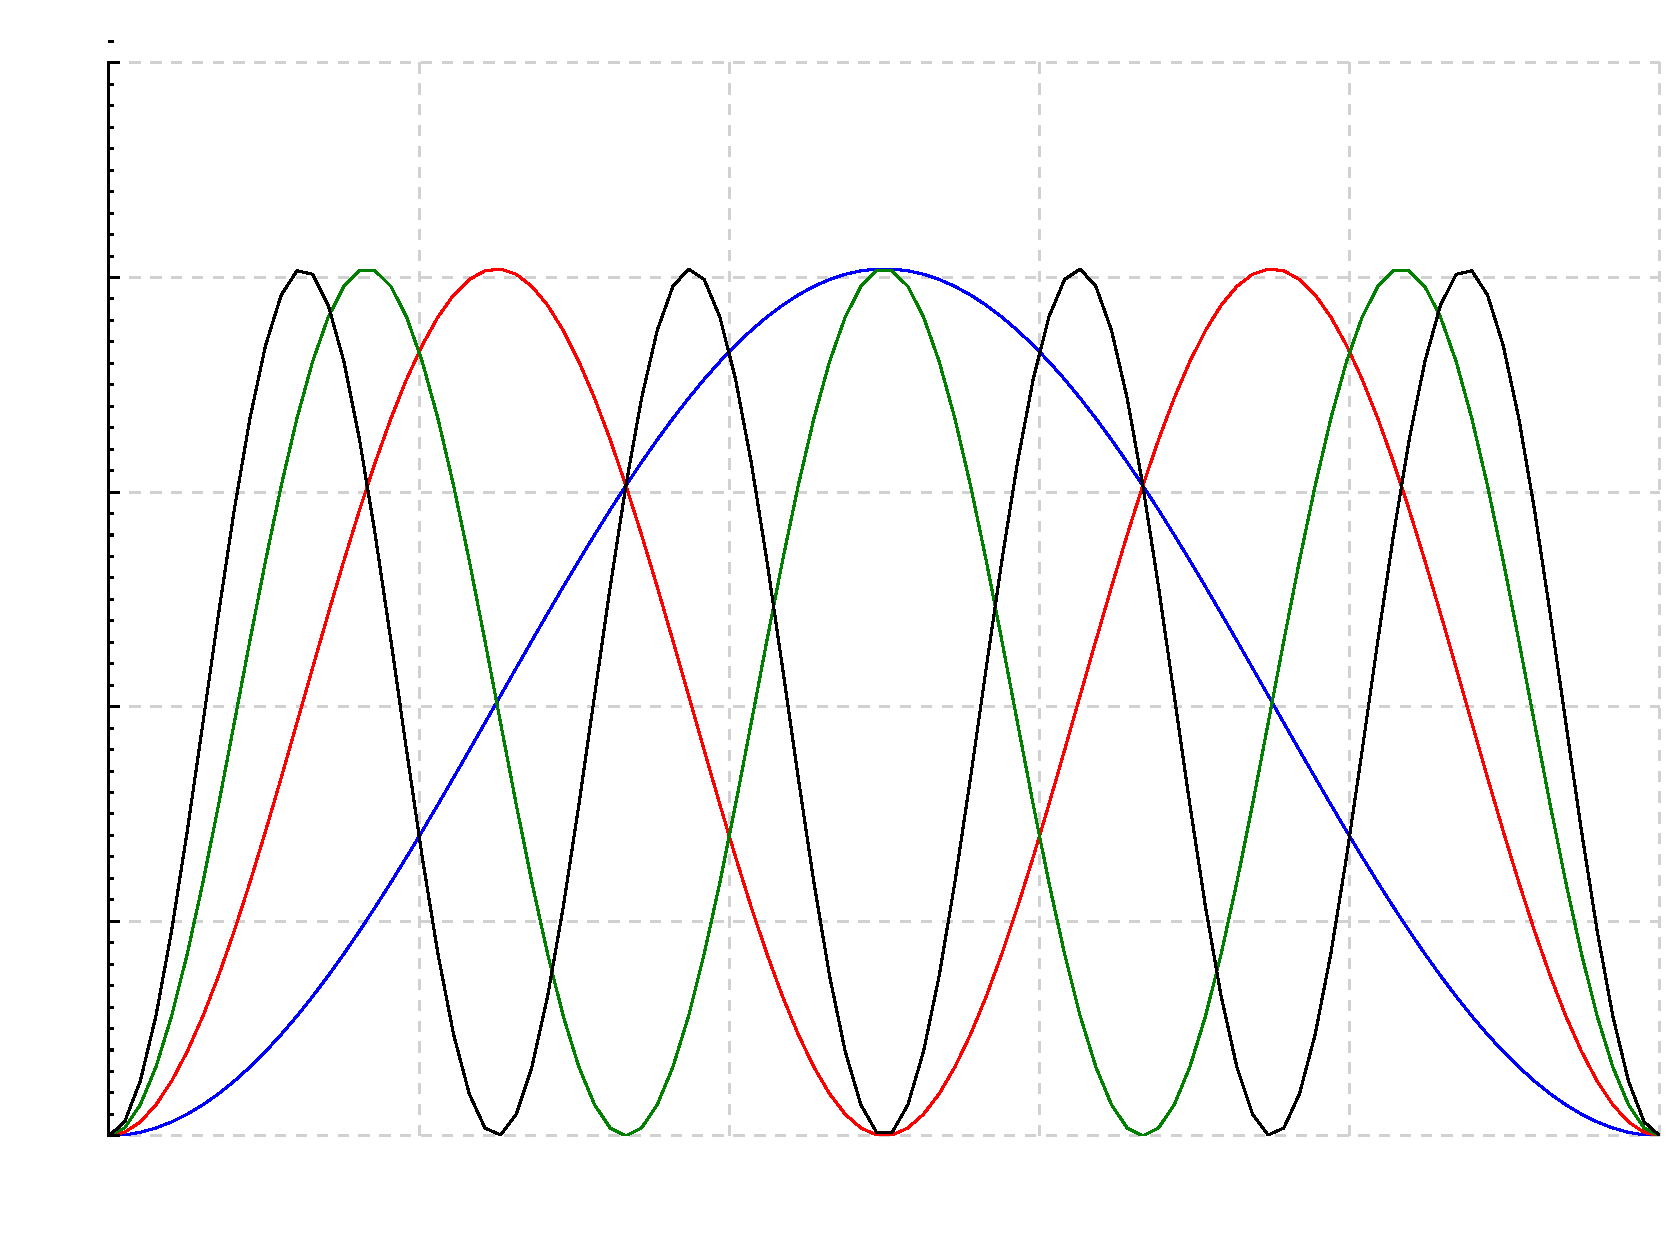
\includegraphics[width=\unitlength,page=1]{figures/eigenfunctions.pdf}}%
    \put(0.004,0.57681454){\color[rgb]{0,0,0}\makebox(0,0)[lb]{\smash{$0.02$}}}%
    \put(0,0){\includegraphics[width=\unitlength,page=2]{figures/eigenfunctions.pdf}}%
    \put(0.0,0.44990405){\color[rgb]{0,0,0}\makebox(0,0)[lb]{\smash{$0.015$}}}%
    \put(0.004,0.32290405){\color[rgb]{0,0,0}\makebox(0,0)[lb]{\smash{$0.01$}}}%
    \put(0.0,0.70690405){\color[rgb]{0,0,0}\makebox(0,0)[lb]{\smash{$0.025$}}}%
    \put(0.004,0.06340405){\color[rgb]{0,0,0}\makebox(0,0)[lb]{\smash{$0$}}}%
    \put(0.004,0.19197949){\color[rgb]{0,0,0}\makebox(0,0)[lb]{\smash{$0.05$}}}%
    \put(0.03773901,0.04840405){\color[rgb]{0,0,0}\makebox(0,0)[lb]{\smash{$0$}}}%
    \put(0.23223901,0.04){\color[rgb]{0,0,0}\makebox(0,0)[lb]{\smash{$0.2$}}}%
    \put(0.41073901,0.03){\color[rgb]{0,0,0}\makebox(0,0)[lb]{\smash{$0.4$}}}%
    \put(0.59823901,0.03){\color[rgb]{0,0,0}\makebox(0,0)[lb]{\smash{$0.6$}}}%
    \put(0.783239,0.03){\color[rgb]{0,0,0}\makebox(0,0)[lb]{\smash{$0.8$}}}%
    \put(0.970739,0.03){\color[rgb]{0,0,0}\makebox(0,0)[lb]{\smash{$1$}}}%
    \put(0.04823902,0.02040406){\color[rgb]{0,0,0}\makebox(0,0)[lb]{\smash{$\psi_1$}}}%
    \put(0.13614134,0.0200705){\color[rgb]{0,0,0}\makebox(0,0)[lb]{\smash{$\psi_2$}}}%
    \put(0.21064144,0.02057045){\color[rgb]{0,0,0}\makebox(0,0)[lb]{\smash{$\psi_3$}}}%
    \put(0.29614145,0.01957047){\color[rgb]{0,0,0}\makebox(0,0)[lb]{\smash{$\psi_4$}}}%
    \put(0.4752763,0.73714841){\color[rgb]{0,0,0}\makebox(0,0)[lb]{\smash{Eigenfunctions}}}%
  \end{picture}%
\endgroup%
}
	\caption{Propability densities for the calculated eigenfunctions $\psi_n$, with the method of finite differences and a grid of $N=100$ for $n = 1,2,3$ and $4$ in one dimension. For simplicity the pre-factor $\frac{\hbar^2}{2m}$ was set to one, obtaining non-normalized eigenfunctions.}
	\label{fig:eigenfunctions}
\end{figure} 
To reduce the problem of a particle in three dimensions to a simple matrix equation, the spatial wave function $\vec{\psi}$ can be stacked, to obtain a $N^3$ dimensional vector through nested vectors,
\begin{align}
\vec{\psi}_{k,l,m} = \begin{pmatrix}\vec{\psi}_{1,1,m} \\ \vdots \\ \vec{\psi}_{1,N,m} \\ \vdots \\ \vec{\psi}_{N,1,m} \\ \vdots \\ \vec{\psi}_{N,N,m} \end{pmatrix}.
\end{align}

For two dimensions the approximated kinetic energy operator $T$ thus becomes the tridiagonal block matrix
\begin{align}
T \approx  \begin{pmatrix}
4	& -1	&  &  -1	 &     &     &  \scalebox{3}{$0$}  \\
    & \ddots	&     & 		&   \ddots   & 	& \\
    & -1 & 4 &  &  &-1 \\
-1 &      &          & 4     & -1       & & \ddots \\
    & \ddots &     &&    \ddots   &       &  \\
  \scalebox{3}{$0$}   &      & -1       &&         & -1     & 4 \\ 
\end{pmatrix} \text{.}
\end{align}

In figure \ref{fig:2d_eigenfunction} an example of an eigenstate for a particle in a two dimensional box is shown.

\begin{figure}[!htb]
	\Huge
	\hspace*{-1.5in}
	\centering
	\subfigure[$\psi_{12}$, $N=60$.]
		{\resizebox{!}{0.28\textwidth}{%% Creator: Inkscape inkscape 0.91, www.inkscape.org
%% PDF/EPS/PS + LaTeX output extension by Johan Engelen, 2010
%% Accompanies image file '2dn12.pdf' (pdf, eps, ps)
%%
%% To include the image in your LaTeX document, write
%%   \input{<filename>.pdf_tex}
%%  instead of
%%   \includegraphics{<filename>.pdf}
%% To scale the image, write
%%   \def\svgwidth{<desired width>}
%%   \input{<filename>.pdf_tex}
%%  instead of
%%   \includegraphics[width=<desired width>]{<filename>.pdf}
%%
%% Images with a different path to the parent latex file can
%% be accessed with the `import' package (which may need to be
%% installed) using
%%   \usepackage{import}
%% in the preamble, and then including the image with
%%   \import{<path to file>}{<filename>.pdf_tex}
%% Alternatively, one can specify
%%   \graphicspath{{<path to file>/}}
%% 
%% For more information, please see info/svg-inkscape on CTAN:
%%   http://tug.ctan.org/tex-archive/info/svg-inkscape
%%
\begingroup%
  \makeatletter%
  \providecommand\color[2][]{%
    \errmessage{(Inkscape) Color is used for the text in Inkscape, but the package 'color.sty' is not loaded}%
    \renewcommand\color[2][]{}%
  }%
  \providecommand\transparent[1]{%
    \errmessage{(Inkscape) Transparency is used (non-zero) for the text in Inkscape, but the package 'transparent.sty' is not loaded}%
    \renewcommand\transparent[1]{}%
  }%
  \providecommand\rotatebox[2]{#2}%
  \ifx\svgwidth\undefined%
    \setlength{\unitlength}{1669bp}%
    \ifx\svgscale\undefined%
      \relax%
    \else%
      \setlength{\unitlength}{\unitlength * \real{\svgscale}}%
    \fi%
  \else%
    \setlength{\unitlength}{\svgwidth}%
  \fi%
  \global\let\svgwidth\undefined%
  \global\let\svgscale\undefined%
  \makeatother%
  \begin{picture}(1,0.55062912)%
    \put(0,0){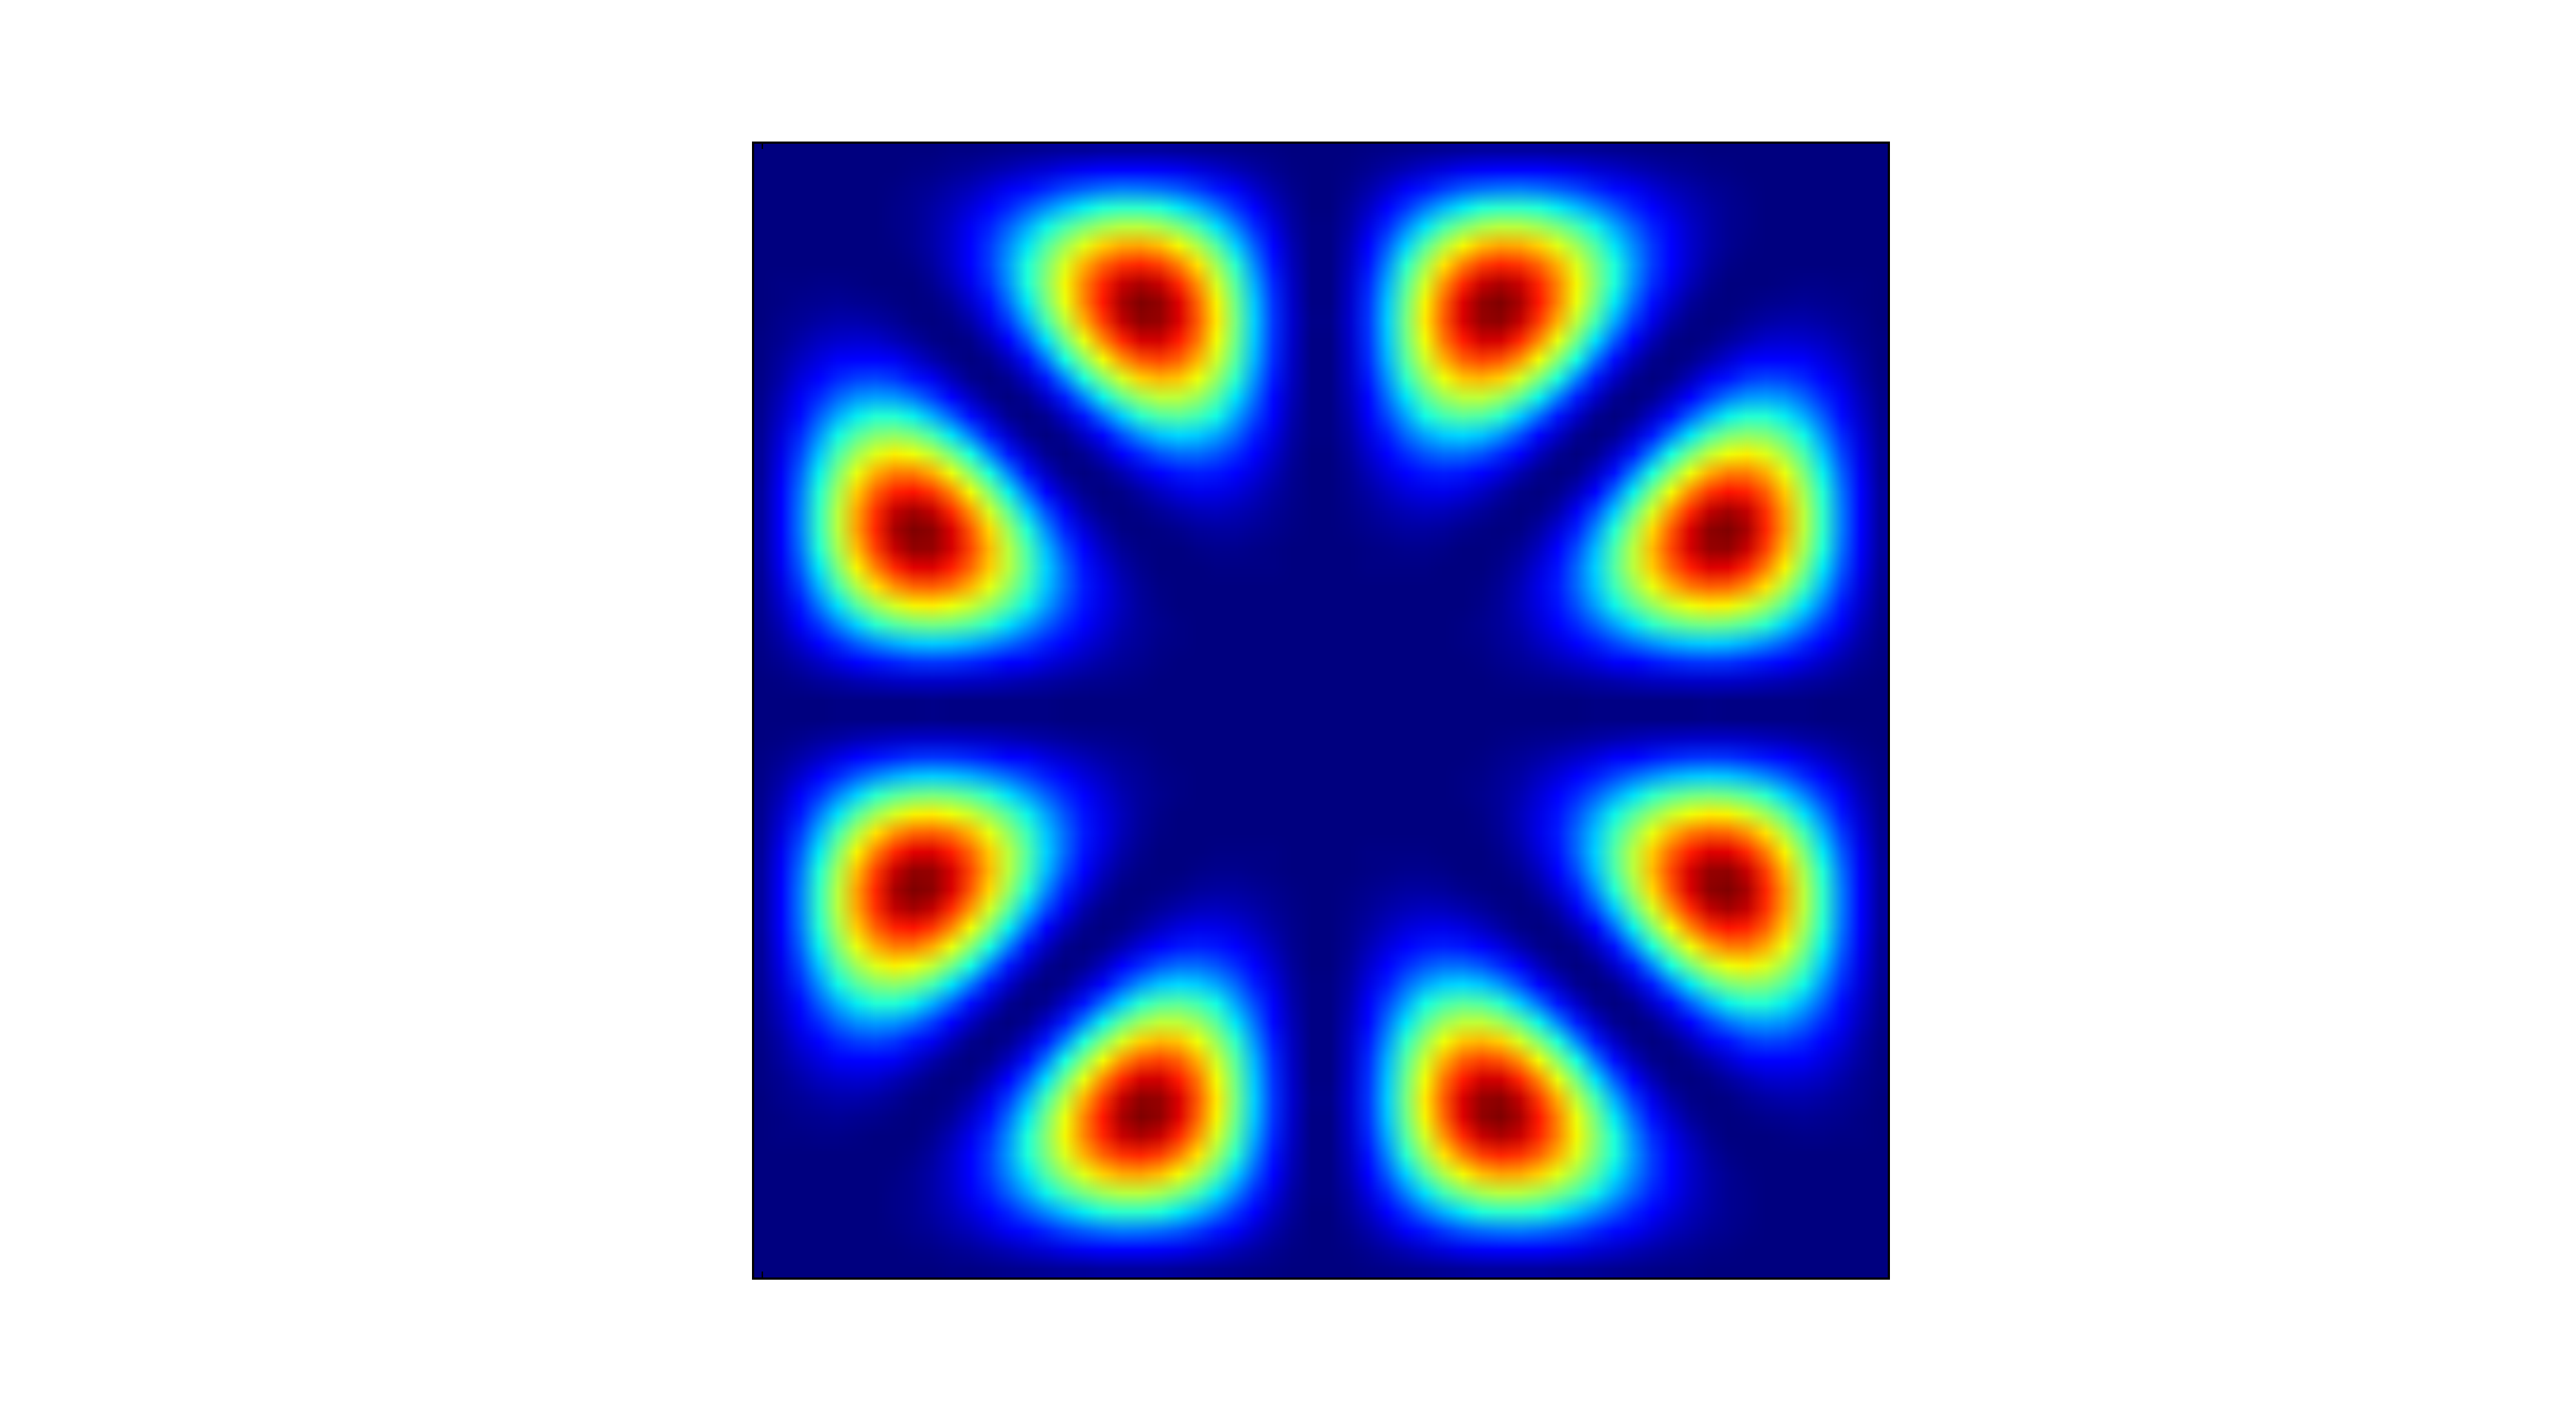
\includegraphics[width=\unitlength,page=1]{figures/2dn12.pdf}}%
    \put(0.29029359,0.02){\color[rgb]{0,0,0}\makebox(0,0)[lb]{\smash{$0$}}}%
    \put(0,0){\includegraphics[width=\unitlength,page=2]{figures/2dn12.pdf}}%
    \put(0.36680651,0.02){\color[rgb]{0,0,0}\makebox(0,0)[lb]{\smash{$0.17$}}}%
    \put(0.4426603,0.02){\color[rgb]{0,0,0}\makebox(0,0)[lb]{\smash{$0.33$}}}%
    \put(0.48651887,0.0524266){\color[rgb]{0,0,0}\makebox(0,0)[lb]{\smash{}}}%
    \put(0.51581787,0.02){\color[rgb]{0,0,0}\makebox(0,0)[lb]{\smash{$0.5$}}}%
    \put(0.58897543,0.02){\color[rgb]{0,0,0}\makebox(0,0)[lb]{\smash{$0.67$}}}%
    \put(0.66133219,0.02){\color[rgb]{0,0,0}\makebox(0,0)[lb]{\smash{$0.83$}}}%
    \put(0.7287978,0.02){\color[rgb]{0,0,0}\makebox(0,0)[lb]{\smash{$1$}}}%
    \put(0.25,0.11614262){\color[rgb]{0,0,0}\makebox(0,0)[lb]{\smash{$0.17$}}}%
    \put(0.25,0.19155608){\color[rgb]{0,0,0}\makebox(0,0)[lb]{\smash{$0.33$}}}%
    \put(00.25,0.2640038){\color[rgb]{0,0,0}\makebox(0,0)[lb]{\smash{$0.5$}}}%
    \put(0.25,0.33941722){\color[rgb]{0,0,0}\makebox(0,0)[lb]{\smash{$0.67$}}}%
    \put(00.25,0.41313597){\color[rgb]{0,0,0}\makebox(0,0)[lb]{\smash{$0.83$}}}%
    \put(0.25,0.48897306){\color[rgb]{0,0,0}\makebox(0,0)[lb]{\smash{$1$}}}%
    \put(0,0){\includegraphics[width=\unitlength,page=3]{figures/2dn12.pdf}}%
    \put(0.25,0.04920264){\color[rgb]{0,0,0}\makebox(0,0)[lb]{\smash{$0$}}}%
    \put(0.51560752,0){\color[rgb]{0,0,0}\makebox(0,0)[lb]{\smash{$x$}}}%
    \put(0.17751812,0.24572913){\color[rgb]{0,0,0}\makebox(0,0)[lb]{\smash{$y$}}}%
  \end{picture}%
\endgroup%
}\label{fig:2d_eigenfunction}}
	%\hfill
	\subfigure[$\psi_{34}$, $N=100$.]
		{\resizebox{0.48\textwidth}{!}{\includegraphics{figures/2dn34_surf.pdf}}\label{fig:2d_surf_eigenfunction}}\\
	 %\hfill
	\caption{Propability densities for the calculated eigenfunctions with the method of finite differences and a grid of $N=100$ and $N=60$ in two dimensions. For simplicity the pre-factor $\hbar^2 /2m$ was set to one, obtaining non-normalized eigenfunctions.}
	\label{Aufbauskizze}
\end{figure}

An implementation of this eigenvalue problem can be done in the following way:
\begin{code}
--index function
index :: (Int, Int) -> Int -> Double
index (i,j) n
	| i == j       =  4
	| i == j + n   = -1
	| i == j - n   = -1
	| i == j + 1   = -1
	| i == j - 1   = -1
	| otherwise    =  0

-- Laplace Matrix in 2 dimensions
t :: Matrix Double
t = buildMatrix (n*n) (n*n) (\(i,j) -> index (i,j) n)	

--Compute eigenvalues and corresponding eigenvectors 
e = sort(toList(mapVector realPart (fst(eig(t)))))
psi = toColumns (mapMatrix realPart (snd(eig(t))))
\end{code}


%\begin{figure}[!htb]
%	\Huge
%	\centering
%	\resizebox{!}{0.7\textwidth}{%% Creator: Inkscape inkscape 0.91, www.inkscape.org
%% PDF/EPS/PS + LaTeX output extension by Johan Engelen, 2010
%% Accompanies image file '2dn12.pdf' (pdf, eps, ps)
%%
%% To include the image in your LaTeX document, write
%%   \input{<filename>.pdf_tex}
%%  instead of
%%   \includegraphics{<filename>.pdf}
%% To scale the image, write
%%   \def\svgwidth{<desired width>}
%%   \input{<filename>.pdf_tex}
%%  instead of
%%   \includegraphics[width=<desired width>]{<filename>.pdf}
%%
%% Images with a different path to the parent latex file can
%% be accessed with the `import' package (which may need to be
%% installed) using
%%   \usepackage{import}
%% in the preamble, and then including the image with
%%   \import{<path to file>}{<filename>.pdf_tex}
%% Alternatively, one can specify
%%   \graphicspath{{<path to file>/}}
%% 
%% For more information, please see info/svg-inkscape on CTAN:
%%   http://tug.ctan.org/tex-archive/info/svg-inkscape
%%
\begingroup%
  \makeatletter%
  \providecommand\color[2][]{%
    \errmessage{(Inkscape) Color is used for the text in Inkscape, but the package 'color.sty' is not loaded}%
    \renewcommand\color[2][]{}%
  }%
  \providecommand\transparent[1]{%
    \errmessage{(Inkscape) Transparency is used (non-zero) for the text in Inkscape, but the package 'transparent.sty' is not loaded}%
    \renewcommand\transparent[1]{}%
  }%
  \providecommand\rotatebox[2]{#2}%
  \ifx\svgwidth\undefined%
    \setlength{\unitlength}{1669bp}%
    \ifx\svgscale\undefined%
      \relax%
    \else%
      \setlength{\unitlength}{\unitlength * \real{\svgscale}}%
    \fi%
  \else%
    \setlength{\unitlength}{\svgwidth}%
  \fi%
  \global\let\svgwidth\undefined%
  \global\let\svgscale\undefined%
  \makeatother%
  \begin{picture}(1,0.55062912)%
    \put(0,0){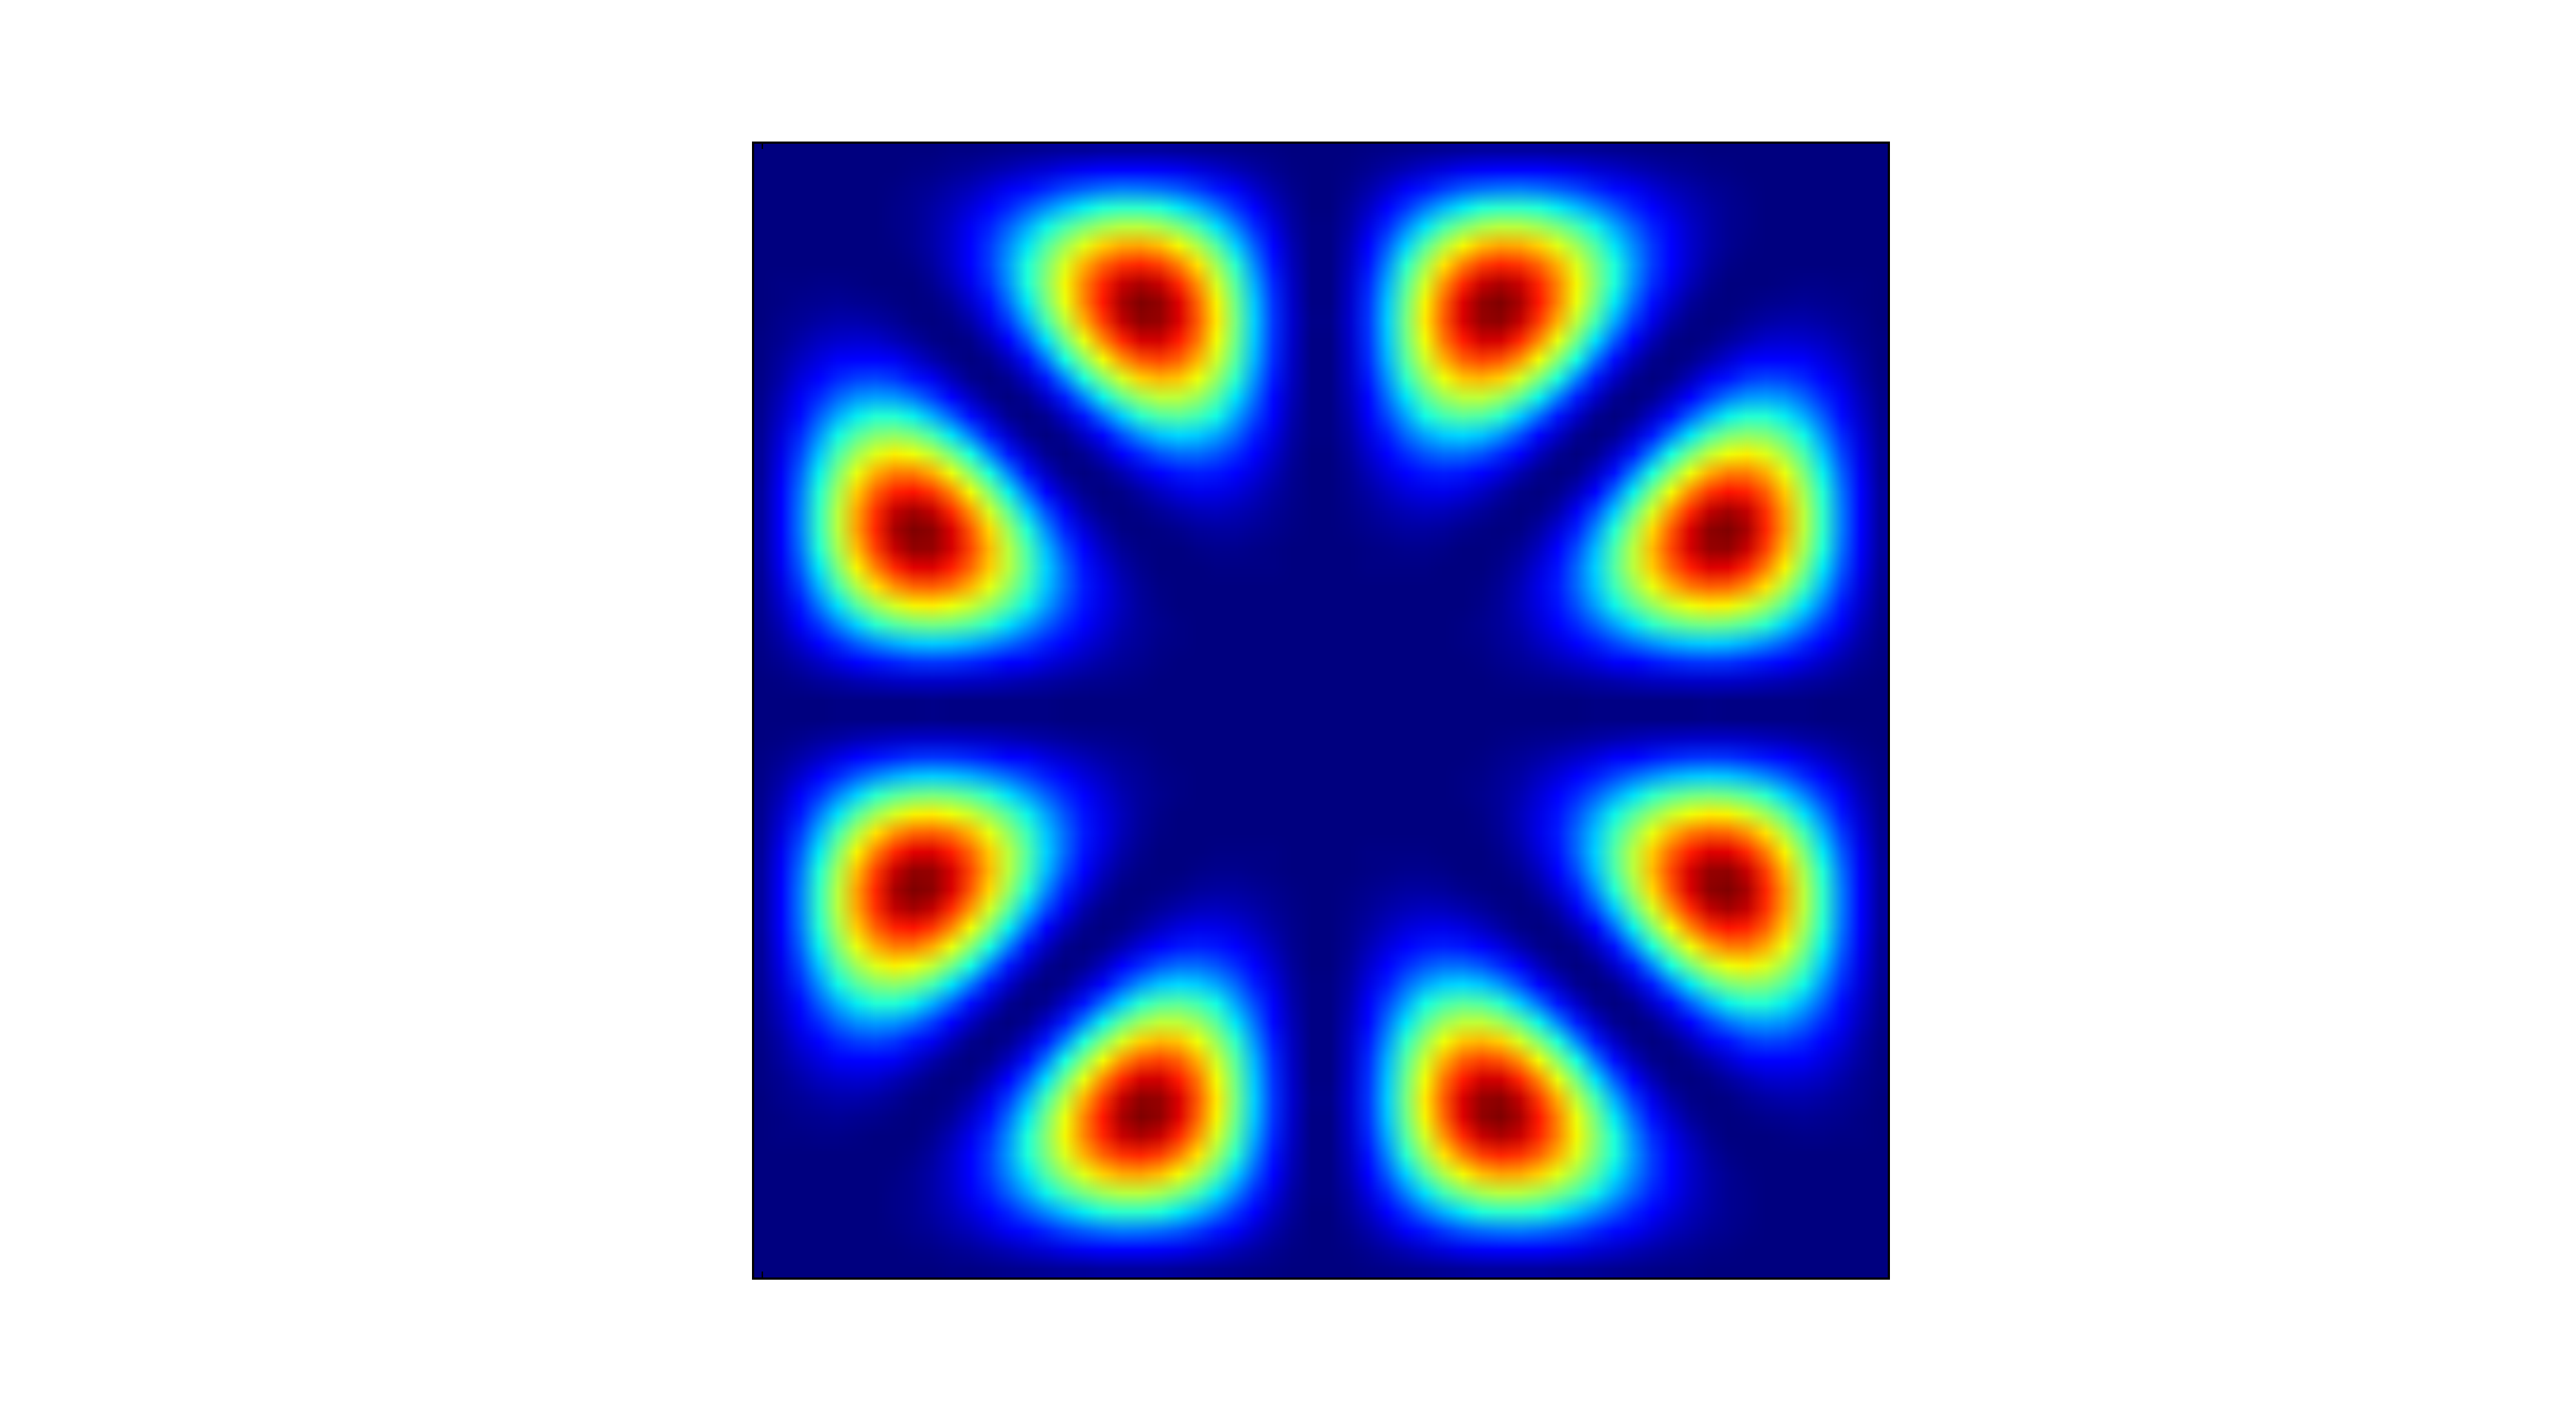
\includegraphics[width=\unitlength,page=1]{figures/2dn12.pdf}}%
    \put(0.29029359,0.02){\color[rgb]{0,0,0}\makebox(0,0)[lb]{\smash{$0$}}}%
    \put(0,0){\includegraphics[width=\unitlength,page=2]{figures/2dn12.pdf}}%
    \put(0.36680651,0.02){\color[rgb]{0,0,0}\makebox(0,0)[lb]{\smash{$0.17$}}}%
    \put(0.4426603,0.02){\color[rgb]{0,0,0}\makebox(0,0)[lb]{\smash{$0.33$}}}%
    \put(0.48651887,0.0524266){\color[rgb]{0,0,0}\makebox(0,0)[lb]{\smash{}}}%
    \put(0.51581787,0.02){\color[rgb]{0,0,0}\makebox(0,0)[lb]{\smash{$0.5$}}}%
    \put(0.58897543,0.02){\color[rgb]{0,0,0}\makebox(0,0)[lb]{\smash{$0.67$}}}%
    \put(0.66133219,0.02){\color[rgb]{0,0,0}\makebox(0,0)[lb]{\smash{$0.83$}}}%
    \put(0.7287978,0.02){\color[rgb]{0,0,0}\makebox(0,0)[lb]{\smash{$1$}}}%
    \put(0.25,0.11614262){\color[rgb]{0,0,0}\makebox(0,0)[lb]{\smash{$0.17$}}}%
    \put(0.25,0.19155608){\color[rgb]{0,0,0}\makebox(0,0)[lb]{\smash{$0.33$}}}%
    \put(00.25,0.2640038){\color[rgb]{0,0,0}\makebox(0,0)[lb]{\smash{$0.5$}}}%
    \put(0.25,0.33941722){\color[rgb]{0,0,0}\makebox(0,0)[lb]{\smash{$0.67$}}}%
    \put(00.25,0.41313597){\color[rgb]{0,0,0}\makebox(0,0)[lb]{\smash{$0.83$}}}%
    \put(0.25,0.48897306){\color[rgb]{0,0,0}\makebox(0,0)[lb]{\smash{$1$}}}%
    \put(0,0){\includegraphics[width=\unitlength,page=3]{figures/2dn12.pdf}}%
    \put(0.25,0.04920264){\color[rgb]{0,0,0}\makebox(0,0)[lb]{\smash{$0$}}}%
    \put(0.51560752,0){\color[rgb]{0,0,0}\makebox(0,0)[lb]{\smash{$x$}}}%
    \put(0.17751812,0.24572913){\color[rgb]{0,0,0}\makebox(0,0)[lb]{\smash{$y$}}}%
  \end{picture}%
\endgroup%
}
%	\caption{Propability densities for the calculated eigenfunction $\psi_{12}$, with the method of finite differences and a grid of $N=60$ in two dimensions. For simplicity the prefactor $\frac{\hbar^2}{2m}$ was set to one, obtaining a non-normalized eigenfunction.}
%\label{fig:2d_eigenfunction}
%\end{figure} 

In three dimensions, we obtain a $N^3$-dimensional Matrix, for example for $N=2$:
\begin{align*}
T \approx
\tiny
\begin{pmatrix}
 6 & -1 & -1 &  & -1 &  &  & \scalebox{3}{$0$}  \\\\
   -1 & 6 & -1 & -1 &  & -1 &  & \\\\
     -1 & -1 & 6 & -1 & -1 &  & -1 & \\\\
        & -1 & -1 & 6 & -1 & -1 &  & -1\\\\
        -1 &  & -1 & -1 & 6 & -1 & -1 & \\\\
           & -1 &  & -1 & -1 & 6 & -1 & -1\\\\
             &  & -1 &  & -1 & -1 & 6 & -1\\\\
              \scalebox{3}{$0$}  &  &  & -1 &  & -1 & -1 & 6\\\\
              \end{pmatrix}
\end{align*}

Referring back to the time expansion in chapter \ref{1}, the time evolution of an eigenfunction of the Hamiltonian is trivial, since $\psi_t$ only differs in phase from the initial state $\psi_0$, so ${|\psi_t|}^2$ is time-independent, although linear combinations of eigenfunctions depend on time, which will not be calculated here.\\

If we take the computing time into account, it is obvious that even with a small grid size $N<100$ and parallelized computing the simulation of a particle in a square well potential leads to unexecutable applications. The increase of dimensions with constant gridsize results in a growing computing time higher than $\mathcal O (t_0^n)$. \\

To proceed to coupled quantum mechanical systems it seems to be mandatory to use efficient approximations.




\section{The Hartree-Fock Method}\label{CH:HF}
    
We consider a real physical system, where particles are not independent, like in atoms, ions, molecules, etc. Assuming the system consists only of $K$ nuclei and $N$ electrons, the Hamiltonian consists of the terms
\begin{align*}
    H = T_i + T_n+ V_{ii} + V_{in} + V_{nn} \text{ ,}
\end{align*} 
where $T_i $ and $T_n$ are the kinetic energies of the electrons and nuclei, respectively. $V_{ii}$ represents the Coulomb repulsion between electrons, $V_{nn}$ between the nuclei and $V_{in}$  the attraction between electrons and nuclei. So the Hamiltonian reads
\begin{align*}
    H &= \sum_{i=1}^N \frac{p_i^2}{2m} + \sum_{n=1}^K \frac{P_n^2}{2M_n} + \frac{1}{4\pi \epsilon_0}\frac{1}{2}\sum_{i,j\neq 1, i \neq j}^N \frac{e^2}{|\mathbf{r}_i - \mathbf{r}_j|} \\ &-  \frac{1}{4\pi \epsilon_0}\sum_{i=1}^K \sum_{i=1}^N \frac{Z_n e^2}{|\mathbf{r}_j-\mathbf{R}_n|} +  \frac{1}{4\pi \epsilon_0}\frac{1}{2} \sum_{n,n'=1;n\neq n'}^K \frac{Z_n Z_{n'} e^2}{|\mathbf{R}_n - \mathbf{R}_{n'}|} \text{,}
\end{align*} where $m$ is the electron mass and $M_n$ the nuclei mass. The index $i$ refers to the electrons, the index $n$ to the nuclei.
This hamiltonian describing the system looks quite complicated and in fact, computing the dynamics of this system seem to be unsolvable even for a few particles and an efficient super computer. Therefore, approximations must be made, still comprising the important information about the system. One approach is the Born-Oppenheimer approximation. It uses the fact that the nuclei are much heavier than the electrons, so the motions of the nuclei are much slower compared to the electrons, justifying to neglect the coulomb repulsion between the nuclei and the kinetic energy of the nuclei, so the approximated Hamiltonian becomes
\begin{align}\label{eq:H_BO}
H_\text{BO} = \sum_{i=1}^N \frac{p_i^2}{2m}  + \frac{1}{4\pi \epsilon_0}\frac{1}{2}\sum_{i,j = 1, i \neq j}^N \frac{e^2}{|\mathbf{r}_i - \mathbf{r}_j|} -  \frac{1}{4\pi \epsilon_0}\sum_{i=1}^K \sum_{i=1}^N \frac{Z_n e^2}{|\mathbf{r}_j-\mathbf{R}_n|}  \text{.}
\end{align}  
The positions of the nuclei can be varied to find the minimum of the total energy.
\subsection{The Hartree-Fock Method and Equations}
In equation (\ref{eq:H_BO}) the antisymmetry of the fermion wave functions was not taken into account. Fock extended the so called \textit{Hartree equation} by taking antisymmetry into account. This approach is based on introducing antisymmetry of the wavefunction by constructing the so called Slater determinant, which is a determinant from single-particle wave functions:
\begin{align*}
\Psi_\text{AS}(\mathbf{x}_1, \dots, \mathbf{x}_N) = \frac{1}{\sqrt{N!}}
\begin{vmatrix}
\psi_1(\mathbf{x}_1) &\psi_2(\mathbf{x}_1)& \dots &\psi_N (\mathbf{x}_1) \\
\psi_1(\mathbf{x}_2) &\psi_2(\mathbf{x}_2)& \dots &\psi_N (\mathbf{x}_2) \\
\vdots & \vdots & & \vdots \\
\psi_1(\mathbf{x}_N)& \psi_2(\mathbf{x}_N)& \dots& \psi_N (\mathbf{x}_N)
\end{vmatrix}
\end{align*} 
Interchanging spatial coordinates of two particles thus changes the sign of the slater determinant. It is important to note that the slater determinant already imposes a restriction to the full wave function. Further improvements could be made to also take linear combinations of slater determinants into account.

The derivation of the \textit{Hartree} and \textit{Hartree-Fock equations} will not be given here, since the main aim here is the implementation of the method. Therefore see e.g. \cite[p. 56-60]{Thijssen2007} and \cite[chapter 3]{Jensen2013}. The \textit{Fock operator} is in natural units given by
 \begin{align} \label{eq:hf}
 \mathcal{F}\psi_k = &\left[-\frac{1}{2} \nabla^2 
 - \sum_n \frac{Z_n}{|\mathbf{r}- \mathbf{R}_n|}\right]\psi_k(\mathbf{x}) + \nonumber
 \sum_{l=1}^N \int \text{d}x' |\psi_l(\mathbf{x}')|^2 \frac{1}{|\mathbf{r}-\mathbf{r}'|} \psi_k(\mathbf{x}) \\
&- \sum_{l=1}^N \int \text{d}x' \psi^*(\mathbf{x}')\frac{1}{|\mathbf{r}-\mathbf{r}'|} \psi_k(\mathbf{x}')\psi_l(\mathbf{x})\text{,}
\end{align}
 satisfying the \textit{Hartree-Fock equation}
\begin{align*}
\mathcal{F} \psi_k = \epsilon_k \psi_k \text{.}
\end{align*} The fourth term in equation (\ref{eq:hf}) is called the exchange term \cite[p. 55]{Thijssen2007} and is nonlocal since the operator is acting on $\psi_k$, but the value at the position $\mathbf{r}$ is determined by the value assumed by $\psi_k$ at all possible positions $\mathbf{r}'$. The eigenvalues $\epsilon_k$ of the Fock operator are related to the total energy by
 \begin{align*}
 E &= \frac{1}{2} \sum_k [\epsilon_k + \braket{\psi_k|h|\psi_k}] \text{, with}\\
 \braket{\psi_k|h|\psi_k} &= \int \text{d}^3\mathbf{x}\; \psi_k^*(\mathbf{x}) \left[-\frac{1}{2} \nabla^2 
 - \sum_n \frac{Z_n}{|\mathbf{r}- \mathbf{R}_n|}\right] \psi_k(\mathbf{x}) \text{.}
 \end{align*} It is obvious that the Fock operator in equation (\ref{eq:hf}) which acts on $\psi_k$ also depends on $\psi_k$ itself.
    
    
    
    
\subsection{The Roothaan Equation}\label{subseq:roothaan}
For molecules numerical basis sets are not efficient, so we use atom centered basis sets to describe the molecular orbital
\begin{align}\label{eq:orbital}
    \psi_k(\vec{x}) = \sum_{p=1}^M C_{pk} \chi_p (\vec{x})\text{,}
\end{align}
with $k = 1,\dots, M$, where $M$ is the number of basis states.
So the Hartree-Fock equation reads
\begin{align*}
    \mathcal{F} (\vec{x})   \psi_k(\vec{x}) &= \epsilon_k    \psi_k(\vec{x})\text{.} \quad \text{Using Eq. (\ref{eq:orbital}) yields}\\
    \mathcal{F} (\vec{x})  \sum_{p=1}^M C_{pk} \chi_p (\vec{x}) &= \epsilon_k \sum_{p=1}^M C_{pk} \chi_p (\vec{x})\text{.}\\
\end{align*}
We can now multiply from the left by a specific basis function $\chi_\nu$. Integrating over the space yields
\begin{align*}
     \sum_{p=1}^M C_{pk} \int \chi_\nu^*(\vec{x})  \mathcal{F} (\vec{x}) \chi_p(\vec{x})\text{d}^3 \vec{x} & =  \epsilon_k  \sum_{p=1}^M C_{pk} \int \chi_\nu^*(\vec{x}) \chi_p(\vec{x})\text{d}^3 \vec{x}   \text{.}
\end{align*}
This can be written in matrix notation of the Hartree-Fock equations, expressed in the atomic orbital basis:
\begin{align}\label{eq:roothaaneq}
    \sum_{p=1}^M C_{pk} F_{\nu p}  &= \epsilon_k \sum_{p=1}^M C_{pk} S_{\nu p}\nonumber\\
    \mathbf{F} \mathbf{C_k} &= \epsilon_k \mathbf{S} \mathbf{C_k} \; \text{,}
\end{align} which is called the \textit{Roothaan equation}.
Since the Fock operator itself depends on $\mathbf{C_k}$ we have the problem of self consistency, because $\mathcal{F}$ has the solution already inside. The Self Consistent Field Method (SCF) uses the approach to solve the above equation iteratively, until the solution deviates only small from the next iteration.
\par Equation (\ref{eq:roothaaneq}) looks similar to the Hartree-Fock equation, but here $\mathbf{S}$ is the overlap matrix for the given orbital basis $\chi_p (\mathbf{r})$. The $\mathbf{S}$-matrix does not vanish, since the used orbital basis does not need to be normalized. In comparison with eq. (\ref{eq:hf}) we can write the Fock matrix as \cite{Thijssen2007}
\begin{align*}
F_{pq} = h_{pq} + \sum\limits_k \sum\limits_{rs} C_{rk}^* C_{sk} \left( 2 \left<pr|g|qs\right> -  \left<pr|g|sq\right> \right)\text{,}
\end{align*} where $h_{pq}$ is identified with the first term of the Fock operator
\begin{align*}
h_{pq} = \left< p|h|q\right> = \int \d^3 r \chi_p^*(\mathbf{r})\left[ -\frac{1}{2} \nabla^2 - \sum\limits_n \frac{Z_n}{\left| \mathbf{R}_n -\mathbf{r} \right|} \right]\chi_q(\mathbf{r})\text{.}
\end{align*} The terms $\left<pr|g|qs\right>$ and $\left<pr|g|sq\right>$ are the two-electron integrals given by
\begin{align*}
\left<pr|g|qs\right> = \int \d^3 r_1 \d^3 r_2 \chi_p^*(\mathbf{r}_1) \chi_r^*(\mathbf{r}_2) \frac{1}{\left| \mathbf{r}_1 -\mathbf{r}_2 \right|} \chi_q(\mathbf{r}_1) \chi_s(\mathbf{r}_2) \text{.}
\end{align*} Here $p$, $q$, $r$ and $s$ label the basis functions and $k$ labels the orbitals $\psi_k$.
For simplicity and implementation it is convenient to define the density matrix as
\begin{align*}
P_{pq} = 2\sum\limits_k C_{pk}^* C_{qk} \text{,}
\end{align*} where the factor $2$ is conventionally due to the spin \cite{Thijssen2007}.
Now the Fock matrix reads
\begin{align*}
F_{pq} = h_{pq} + \sum\limits_{rs} P_{sr} \left( 2 \left<pr|g|qs\right> -  \left<pr|g|sq\right> \right)\text{.}
\end{align*} In this orbital representation the energy is given by
\begin{align*}
E = \sum\limits_{pq} P_{pq}h_{pq} + \frac{1}{2}  \sum\limits_{pqrs} P_{pq}P_{sr} \left[ \left<pr|g|qs\right> -  \frac{1}{2}\left<pr|g|sq\right> \right] \text{.}
\end{align*}

\subsection{Closed and open shell systems}    
Since also the spin plays important role in atomic structures, further restriction on the spin states can be made, leading to closed and open-shell systems, referred to as Unrestricted Hartree-Fock, and Restricted Hartree-Fock. In a closed shell, the orbitals are occupied by two electrons with opposite spin, whereas in an open shell, the energy levels are partially filled where levels contain only one electron. Since the occupied levels in atoms strictly follow the Aufbau principle, the restriction of a closed-shell might lead to unphysical results in some cases. Even if the number of electrons is even, the electrons do not necessarily occupy closed shells -- for an odd number of electrons, an open shell is always present.
For a closed shell, and thus for even $N$, the slater determinant is
\begin{align*}
\Psi_\textbf{R} = \det \left[\alpha \psi_1, \dots, \alpha\psi_{N/2}, \beta \psi_1, \dots, \beta\psi_{N/2} \right] (\mathbf{x}_1, \dots, \mathbf{x}_N) , 
\end{align*} which is referred to as \textbf{restricted closed shell Hartree-Fock} (RHF).
When allowing the number of spin-up and spin-down states to be different, the slater-determinant becomes:
\begin{align*}
\Psi_\textbf{R} = \det \left[\alpha \psi_1, \dots, \alpha\psi_{N_\alpha}, \beta \psi_1, \dots, \beta\psi_{N_\beta} \right] (\mathbf{x}_1, \dots, \mathbf{x}_N).
\end{align*} This represents the \textbf{restricted open shell Hartree-Fock} (ROHF).
However, in the general case, also the one-particle wave functions have spin-dependence, requiring two distinct basis sets, for spin-down and for spin-up states, respectively, yielding to the \textbf{unrestricted Hartree-Fock} (UHF) method, with slater determinant
\begin{align*}
\Psi_\textbf{R} = \det \left[\alpha \psi_1^\alpha, \dots, \alpha\psi_{N_\alpha}^\alpha, \beta \psi_1^\beta, \dots, \beta\psi_{N_\beta}^\beta \right] (\mathbf{x}_1, \dots, \mathbf{x}_N).
\end{align*}
In this general case, the spin-dependence of the basis set is reflected in the expansion coefficients $\mathbf{C}_k$, since they also depend on the spin, yielding the so-called \emph{Pople-Nesbet} equations:
\begin{align*}
\mathbf{F}^\alpha \mathbf{C_k}^\alpha &= \epsilon_k^\alpha \mathbf{S} \mathbf{C_k}^\alpha \\
\mathbf{F}^\beta \mathbf{C_k}^\beta &= \epsilon_k^\beta \mathbf{S} \mathbf{C_k}^\beta
\end{align*}
Here, each equation for spin-up and spin-down orbitals has to be solved independently. However, we will restrict ourselves to RHF for simplicity.

\subsection{Basis set and basis functions}
A key for obtaining reasonable and accurate results in Hartree-Fock theory is the correct choice of the orbital set which on which the calculation is based. As mentioned in section. \ref{subseq:roothaan}, the one-particle wave functions are expanded in the form:
\begin{align*}
    \psi_k(\vec{r}) = \sum_{p=1}^M C_{pk} \chi_p (\vec{r})\text{,}
\end{align*} which is a linear combination of molecular orbitals (LCAO).
Since analytic forms of the desired atomic orbitals are only known for the hydrogen atom, these orbitals need to be approximated in a suitable manner. Following the analytic solution for the hydrogen orbital, we get a general form of atomic orbital basis functions, whith the nucleus centered at $\mathbf{R_\text{A}}$:
\begin{align*}
\chi_\alpha (\mathbf{r}) = r^m P_l (x,y,z) \text{e}^{-\alpha |\mathbf{r-R_\text{A}}|},
\end{align*}, where $\alpha$ defines the range of the orbital. Here, $P_l$ is a polynomial in $x,y$ and $z$ of degree $l$. This orbital type is also known as a Slater type orbital (STO). However, in Hartree-Fock calculations these orbital types are highly disadvantageous, since integrals containing products of STOs are analytically very difficult and in most cases impossible to compute.

Instead, we can avoid this problem, by replacing the simple exponential by a Gaussian function, yielding:
\begin{align*}
\chi_\alpha(\mathbf{r}) = P_M (x,y,z) \text{e}^{-\alpha (\mathbf{r-R_\text{A}})^2}
\end{align*} These functions are called \emph{primitive basis functions}. In this case, products of Gaussian type orbitals (GTO) centered at different nuclei are still Gaussian functions. Thus, the necessary integrals, such as the kinetic integrals, the overlap integrals, the nuclear repulsion integrals as well as the electron-electron interaction integrals can be calculated analytically.
To accurately approximate a Slater-type orbital one can use a linear combination of Gaussian-type orbitals, which is called a \emph{contracted} Gaussian orbital, with contraction coefficients $a_i$. Denoting a primitive Gaussian with $G(\alpha, A, l, m, n)$, a contraction is simply given by a set of primitive Gaussians:
\begin{align*}
G^\text{Contr.} = \sum\limits_i^n a_i G(\alpha_i, A, l, m, n)
\end{align*} 
In Fig. \ref{fig:STO_GTO}, a comparison of different contractions for a 1s orbital is shown. Choosing and finding the right basis set is a rather difficult part and there is a huge data base of different basis sets available (see, e.g. \cite{schuchardt2007basis, feller1996role} and the \href{https://bse.pnl.gov/}{EMSL Basis Set Exchange database}). Here, we use the basis set provided by the EMSL Basis Set Exchange database for our calculations.

For a given basis set, the following integrals need to be computed in the Hartree-Fock method:
\begin{itemize}
\item \textbf{Overlap integral}
\begin{align*}
S_{ij} = \left<\alpha_1, \mathbf{A}, l_1, m_1, n_1 |\alpha_2, \mathbf{B}, l_2, m_2, n_2 \right> = \int \psi_1^*(\mathbf{r})
\psi_2(\mathbf{r})d\mathbf{r}
\end{align*}
\item \textbf{Kinetic energy integral}
\begin{align*}
T_{ij} = \bra{\alpha_1, \mathbf{A}, l_1, m_1, n_1}-\frac{1}{2}\nabla^2\ket{\alpha_2, \mathbf{B}, l_2, m_2, n_2} = \int \psi_1^*(\mathbf{r})\left( -\frac{1}{2}\nabla^2\right)
\psi_2(\mathbf{r})d\mathbf{r}
\end{align*}
\item \textbf{Nuclear Attraction integrals}
\begin{align*}
V_{ij}^C = \bra{\alpha_1, \mathbf{A}, l_1, m_1, n_1}\frac{Z_C}{r_C}\ket{\alpha_2, \mathbf{B}, l_2, m_2, n_2} = \int \psi_1^*(\mathbf{r})\left(\frac{Z_C}{r_C}\nabla^2\right)
\psi_2(\mathbf{r})d\mathbf{r}
\end{align*}
\item \textbf{Electron repulsion integral}
\begin{align*}
\text{ERI} = \left<pr|g|qs\right> = \int \d^3 r_1 \d^3 r_2 \psi_p^*(\mathbf{r}_1) \psi_r^*(\mathbf{r}_2) \frac{1}{\left| \mathbf{r}_1 -\mathbf{r}_2 \right|} \psi_q(\mathbf{r}_1) \psi_s(\mathbf{r}_2)
\end{align*}
\end{itemize} The last integral is by far the most important and also most difficult part since the calculation involving 4 different primitive Gaussians scales with $N^4$, where $N$ is the number of primitive Gaussians. Using very efficient state-of-the-art algorithms, the calculation of the electron repulsion integral can be reduced to $\mathcal{O}(N)$.
For these integrals, analytic solutions exists. The implementation of these integrals is straight-forward but very tedious. For a detailed calculation of Gaussian integral evaluation, see \cite{fermann1997fundamentals, petersson2009detailed, gill1989efficient, huzinaga1985basis, raffenetti1973general}. 


\begin{figure}
\centering
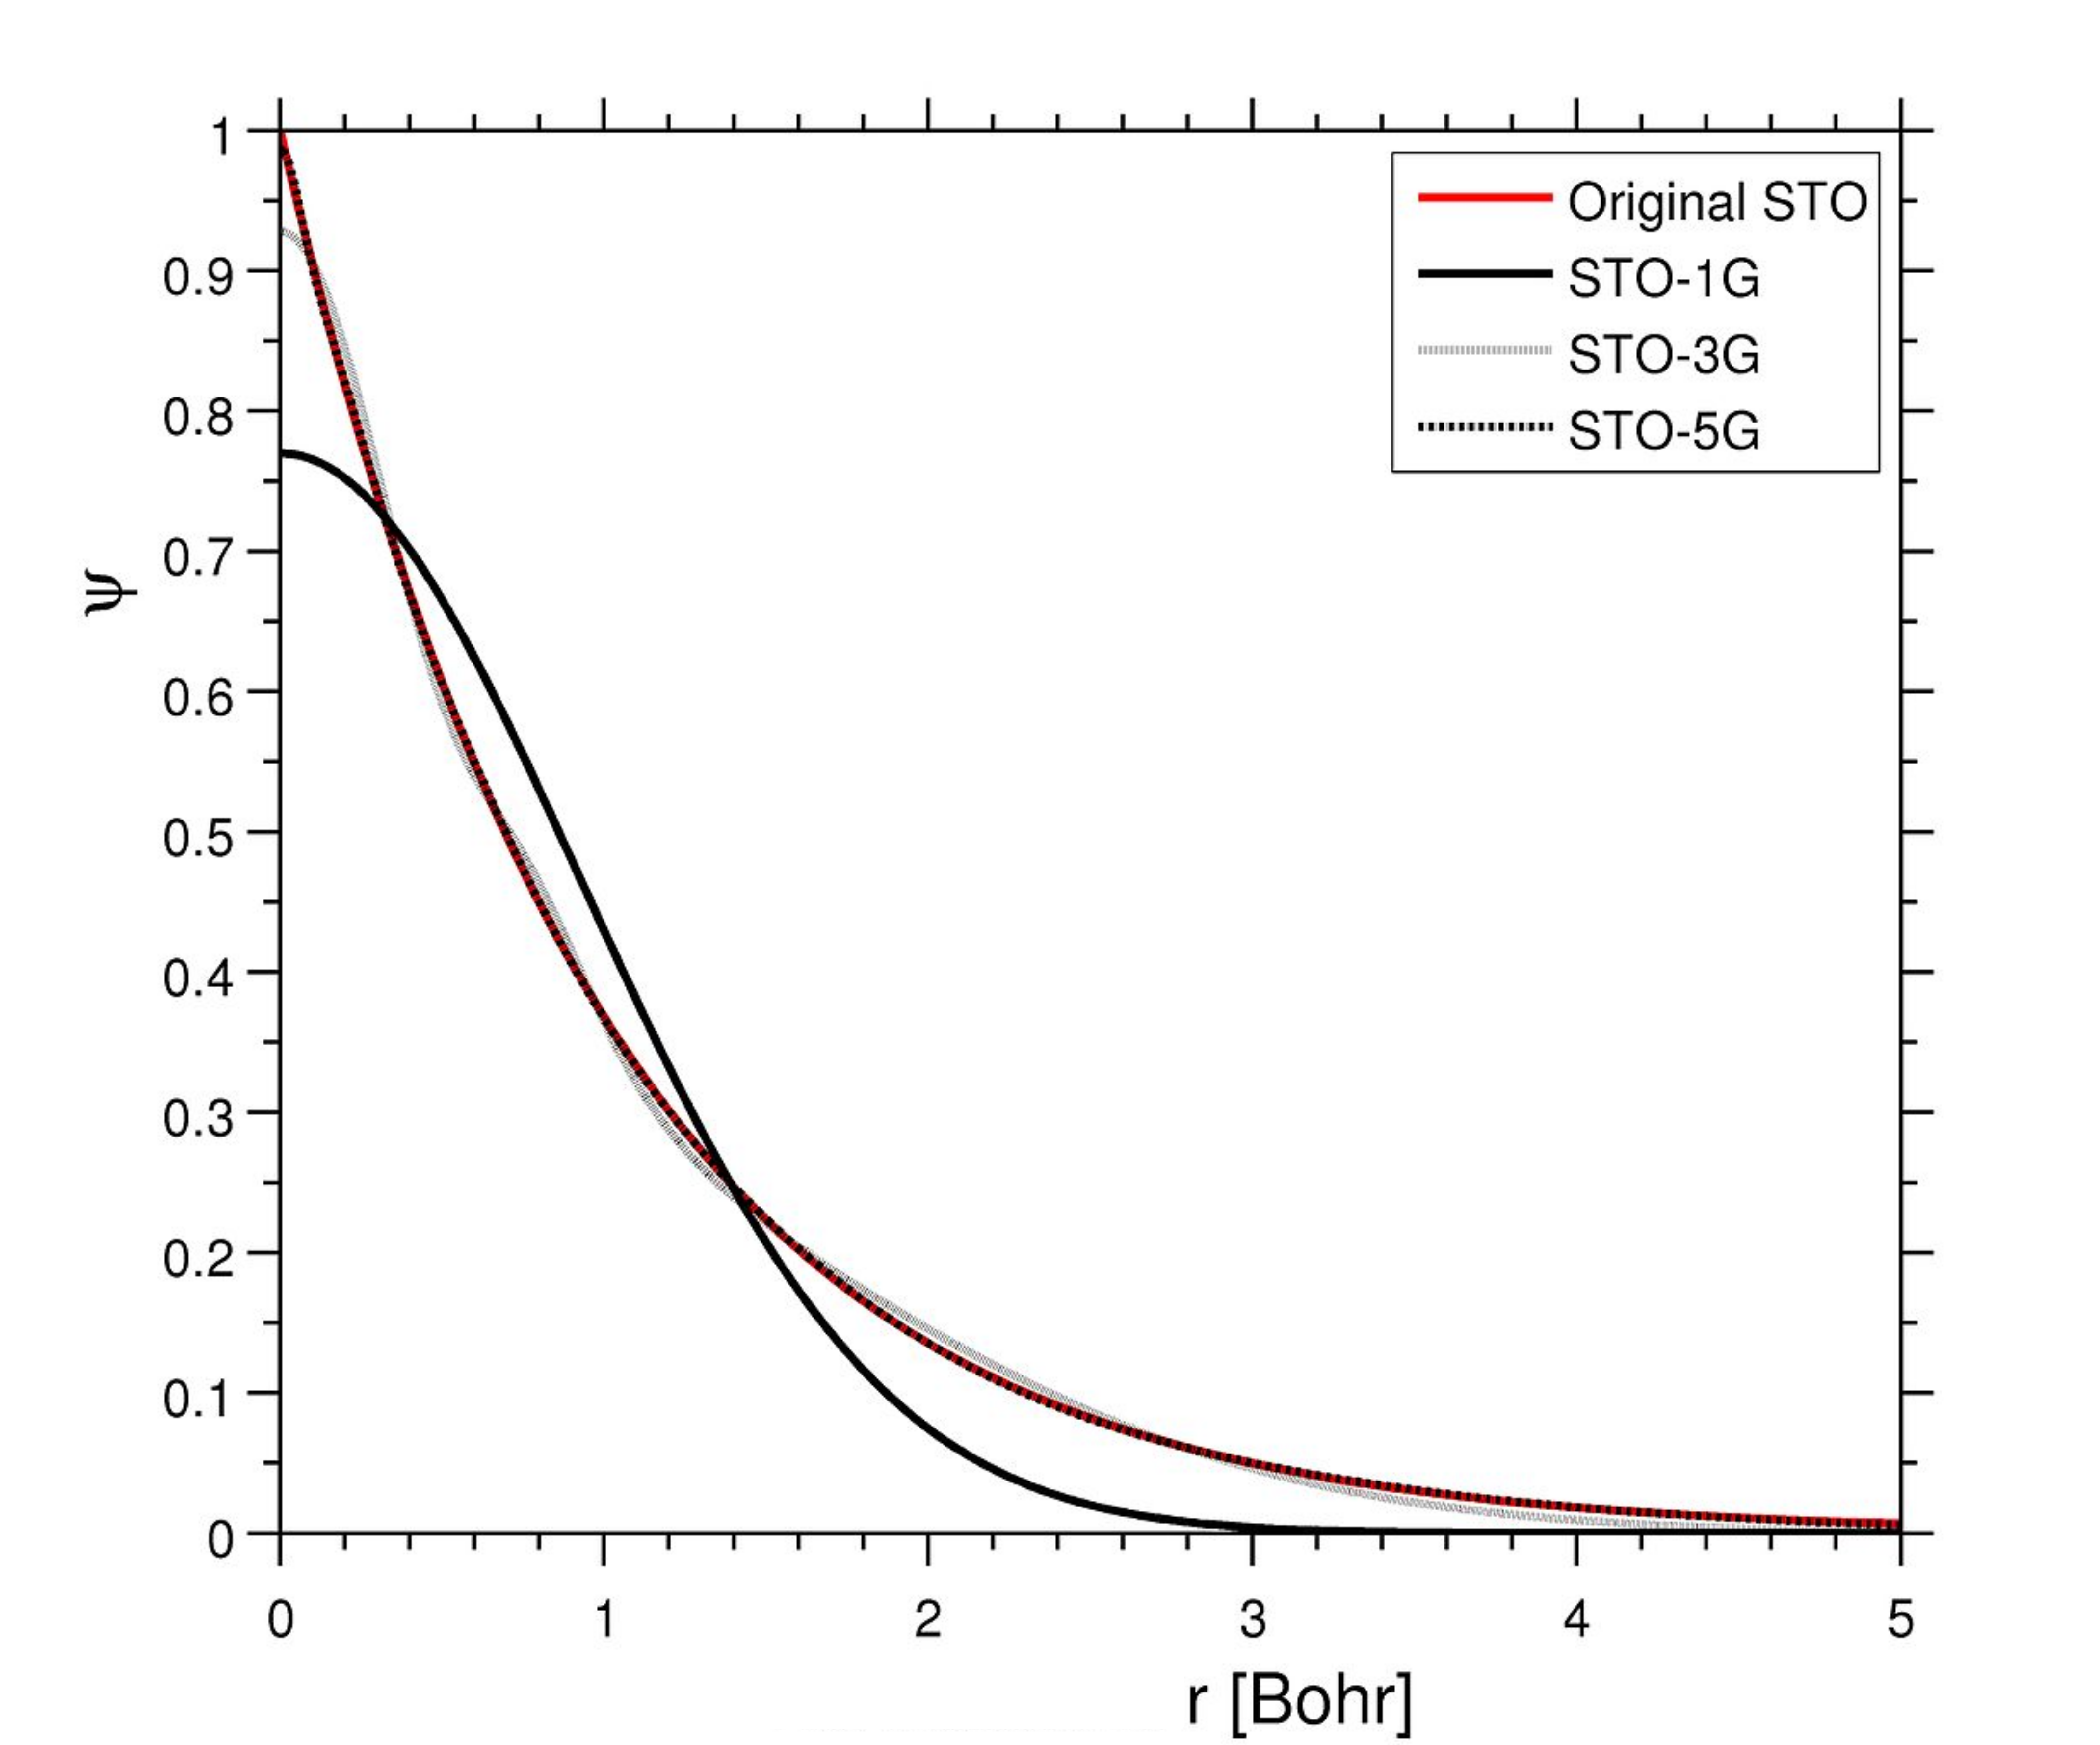
\includegraphics[width=0.5\textwidth]{figures/1228px-Gauss_sto4.png}
\caption{Approximation of a slater determinant for the 1s orbital by STO-1G, STO-3G and STO-6G basis functions. \cite{pict}}
\label{fig:STO_GTO}
\end{figure}

    
\subsection{Program Structure}
Here a general overview of the general program structure will be given.
As outlined before it is important to consider a suitable set of basis functions describing the electrons electrons of the atoms. The accuracy and efficiency of the basis largely depend on the choice of the basis functions, so they need to be chosen carefully. For suitable calculations we use Gaussian basis functions, so the important integrals can be calculated analytically. For a more detailed view on basis functions, see appendix \ref{App:AppendixA}.
Below the program procedure is sketched.

\begin{enumerate}
	\item \textbf{Input data}:\\
	Here the basis sets as well as the geometry of the atoms in the molecule will be provided and parsed to the program. Furthermore the numbers of electrons $N$ and the atomic charge numbers $Z_n$ are needed as input.
	\item \textbf{Calulate independent matrices}\\
	All matrices that are independent of the eigenvectors $\mathbf{C}_k$ can be calculated:
	\begin{itemize}
		\item The overlap matrix $S_pq$,
		\item The two-electron integrals $\braket{pr|g|qs}$,
		\item The uncoupled one-electron Hamiltonian $h_{pq}$.
	\end{itemize}
	\item \textbf{Make an initial guess for the density matrix $\mathbf{P}$.}\\
	A possibility is to use $\mathbf{P} = 0$ as an initial guess, which means that the electrons only feel the nuclei but not each other.
	\item \textbf{Self-consistency procedure}\\
	This program section is the most important, since in solves the Roothaan equation recursively. It consist of the following steps.
	\begin{itemize}
		\item Calculate the Coulomb and exchange contributions to the Fock matrix,
		\item Construct the Fock matrix,
		\item Solve the Roothaan equation by diagonalization of the Fock matrix for the given density matrix $\mathbf{P}$,
		\item With the obtained eigenvectors a new density matrix is $\mathbf{P}$ is constructed.
	\end{itemize}
	\item \textbf{Output data}\\
	The output is are the converged eigenstates $\mathbf{C}_k$ and its corresponding Fock levels.
\end{enumerate}

In figure \ref{skiz:programstructure} a schematic representation of the general program scheme is shown.
\newpage    
    
\tikzstyle{decision} = [diamond, draw, fill=blue!20, text width=7em, text badly centered, node distance=5.7cm, inner sep=0pt]
\tikzstyle{block} = [rectangle, draw, fill=blue!20,  text width=7em, text centered, rounded corners, minimum height=4em]
\tikzstyle{line} = [draw]
\tikzstyle{largeblock} = [rectangle, draw, fill=blue!20, text width=17em, text centered, rounded corners, minimum height=4em]
\tikzstyle{cloud} = [draw, ellipse,fill=red!20, node distance=3cm, minimum height=2em]
\tikzstyle{c} = [rectangle, draw, inner sep=0.5cm, dashed]
\begin{figure}[!htb]
\centering
\scalebox{0.8}{   
\begin{tikzpicture}[node distance = 3.3cm, auto]
    % Place nodes
    \node [block] (init) {choose set of basis functions $\chi$};
    \node [block, below of=init] (hpq) {guess density matrix $\mathbf{P}$};
    \node [block, left of=hpq] (Spq) {overlap matrix $S_{pq}$};
    \node [block, right of=hpq] (prgqs) {two-electron integrals $\braket{pr|g|qs}$};
    \node [block, right of=prgqs] (Ppq) {uncoupled one-electron Hamiltonian $h_{pq}$};
    \node [block, below of=Spq] (VSV) {bring $\mathbf{S}$ to unitform, s.th $\mathbf{V^\dagger SV}  = \mathbf{1}$};
    
    \node [largeblock, scale=0.9, below of=prgqs] (G) {Coulomb and exchange contributions to the Fock matrix. {\small $G_{pq}=\sum_{rs}P_{rs} \left[\braket{pr|g|qs} - \frac{1}{2} \braket{pr|g|sq}\right]$}};
    \node [block, below left of=G] (F) {Fock matrix \mbox{$F_{pq} = h_{pq} + G_{pq}$}};
    \node [block, below of=F] (diagF) {solving $\mathbf{F C} = \epsilon \mathbf{C}$ by diagonalization of $\mathbf{F}$};
    \node [block, below of=diagF] (newP) {construct  new density matrix through \mbox{$ P_{pq} = 2 \sum C_{pk} C_{pk}^*$}};
     \node [decision, right of=newP] (convergence) {convergence};
     \node [block, below right of=convergence] (done) {done};
     
     \node [c,fit=(G) (newP) (convergence)] (container) {};
 

    
    \path [line] (init) -| (Spq);
    \path [line] (init) -| (Ppq);

    \path [line] (init) -- (hpq);
    \path [line] (init) -| (prgqs);
    \path [line] (Spq) -- (VSV);
    \path [line] (G) |-	 (F);
    \path [line] (F) -- (diagF);
    \path [line] (diagF) -- (newP);
    \path [line] (VSV) |- (newP);
    \path [line] (prgqs) -- (G);
    \path [line] (Ppq) |- (F);
    \path [line] (hpq) |- (G);
    
     \path [line] (newP) |- (convergence);
    \path [line] (convergence) |- node [near start] {no} (G);
    \path [line] (convergence) -| node [near end] {yes} (done); 
    
\end{tikzpicture}
}

\caption{General scheme of the program structure.}
\label{skiz:programstructure}
\end{figure}
\pagebreak
\begin{appendices}
\section{Basis Functions} \label{App:AppendixA}
\end{appendices}
\pagebreak



    % bib stuff
    \nocite{*}
\bibliography{bibfile} 
\end{document}
